
%package list
\documentclass{article}
\usepackage[top=3cm, bottom=3cm, outer=3cm, inner=3cm]{geometry}
\usepackage{graphicx}
\usepackage{url}
%\usepackage{cite}
\usepackage{hyperref}
\usepackage{array}
\usepackage{multicol}
\newcolumntype{x}[1]{>{\centering\arraybackslash\hspace{0pt}}p{#1}}
\usepackage{natbib}
\usepackage{pdfpages}
\usepackage{multirow}
\usepackage{float}
\usepackage[normalem]{ulem}
\useunder{\uline}{\ul}{}
\usepackage{svg}
\usepackage{amsmath}
\usepackage{hyperref}

%%%%%%%%%%%%%%%%%%%%%%%%%%%%%%%%%%%%%%%%%%%%%%%%%%%%%%%%%%%%%%%%%%%%%%%%%%%%
%%%%%%%%%%%%%%%%%%%%%%%%%%%%%%%%%%%%%%%%%%%%%%%%%%%%%%%%%%%%%%%%%%%%%%%%%%%%
\newcommand{\csemail}{vmachacaa@unsa.edu.pe}
\newcommand{\csdocente}{Vicente Machaca Arceda}
\newcommand{\cscurso}{Algoritmos y Estructura de Datos}
\newcommand{\csuniversidad}{Universidad Nacional de San Agustín}
\newcommand{\csescuela}{Maestría en Ciencias de la Computación}
\newcommand{\cspracnr}{04}
\newcommand{\cstema}{Kd-tree}
%%%%%%%%%%%%%%%%%%%%%%%%%%%%%%%%%%%%%%%%%%%%%%%%%%%%%%%%%%%%%%%%%%%%%%%%%%%%
%%%%%%%%%%%%%%%%%%%%%%%%%%%%%%%%%%%%%%%%%%%%%%%%%%%%%%%%%%%%%%%%%%%%%%%%%%%%


\usepackage[english,spanish]{babel}
\usepackage[utf8]{inputenc}
\AtBeginDocument{\selectlanguage{spanish}}
\renewcommand{\figurename}{Figura}
\renewcommand{\refname}{Referencias}
\renewcommand{\tablename}{Tabla} %esto no funciona cuando se usa babel
\AtBeginDocument{%
	\renewcommand\tablename{Tabla}
}

\usepackage{fancyhdr}
\pagestyle{fancy}
\fancyhf{}
\setlength{\headheight}{30pt}
\renewcommand{\headrulewidth}{1pt}
\renewcommand{\footrulewidth}{1pt}
\fancyhead[L]{\raisebox{-0.2\height}{
\includegraphics[width=3cm]{img/logo_unsa}}}
\fancyhead[C]{}
\fancyhead[R]{\fontsize{7}{7}\selectfont	\csuniversidad \\ \csescuela \\ \textbf{\cscurso} }
\fancyfoot[L]{Grupo N◦ 02}
\fancyfoot[C]{\cscurso}
\fancyfoot[R]{Página \thepage}

\begin{document}

\vspace*{10px}

\begin{center}
	\fontsize{17}{17} \textbf{ Práctica \cspracnr}
\end{center}

%\centerline{\textbf{\underline{\Large Título: Informe de revisión del estado del arte}}}
%\vspace*{0.5cm}

\begin{table}[h]
	\begin{tabular}{|x{4.7cm}|x{4.8cm}|x{4.8cm}|}
		\hline
		\textbf{DOCENTE} & \textbf{CARRERA} & \textbf{CURSO} \\
		\hline
		\csdocente       & \csescuela       & \cscurso       \\
		\hline
	\end{tabular}
\end{table}

\begin{table}[h]
	\begin{tabular}{|x{4.7cm}|x{4.8cm}|x{4.8cm}|}
		\hline
		\textbf{PRÁCTICA} & \textbf{TEMA} & \textbf{DURACIÓN} \\
		\hline
		\cspracnr         & \cstema       & --                \\
		\hline
	\end{tabular}
\end{table}

\section{Integrantes}
\begin{itemize}
	\item Grupo N° 2
	\item Integrantes:
	      \begin{itemize}
		      \item EDER ALONSO AMPUERO ATAMARI
		      \item HOWARD FERNANDO ARANZAMENDI MORALES
		      \item JOSE EDISON PEREZ MAMANI
		      \item HENRRY IVAN ARIAS MAMANI
	      \end{itemize}
\end{itemize}

\section{Repositorio GitHub}
URL Github: \href{https://github.com/hAriasm/Practica4_ayed}{Repositorio Práctica 4 AyED}

\section{Marco Teórico}
\subsection{Kd-Tree}
\subsection{KNN}
\section{Ejercicios}
\subsection{Ejercicio N}
\subsubsection{Definición}
\paragraph{}
Un árbol K-D (también llamado árbol K-dimensional) es un árbol de búsqueda binaria donde los datos en cada nodo son un punto K-dimensional en el espacio. En resumen, es una estructura de datos de partición de espacio (detalles a continuación) para organizar puntos en un espacio K-Dimensional.

Un nodo que no es una hoja en el árbol K-D divide el espacio en dos partes, llamadas medios espacios.

Los puntos a la izquierda de este espacio están representados por el subárbol izquierdo de ese nodo y los puntos a la derecha del espacio están representados por el subárbol derecho. Pronto estaremos explicando el concepto de cómo se divide el espacio y se forma el árbol.

En aras de la simplicidad, entendamos un árbol 2-D con un ejemplo.

La raíz tendría un plano alineado con el eje x, los hijos de la raíz tendrían ambos planos alineados con el eje y, los nietos de la raíz tendrían todos planos alineados con el eje x, y los bisnietos de la raíz tendrían todos planos alineados con el eje y, y así sucesivamente.

\subsubsection{Generalización}
\paragraph{}
Numeremos los planos como 0, 1, 2, …(K – 1). Del ejemplo anterior, es bastante claro que un punto (nodo) en la profundidad D tendrá un plano alineado donde A se calcula como:

A = D mod K
\subsubsection{¿Cómo determinar si un punto estará en el subárbol izquierdo o en el subárbol derecho?}
\paragraph{}
Si el nodo raíz esta alineado en el plano A, el subárbol izquierdo contendrá todos los puntos cuyas coordenadas en ese plano sean más pequeñas que las del nodo ráiz. De manera similar, el subárbol derecho contendrá todos los puntos cuyas coordenadas en ese plano sean mayores-iguales que las del nodo raíz.

\subsubsection{Creación de un árbol 2-D}
\paragraph{}
Considere los siguientes puntos en un plano 2-D:
(3, 6), (17, 15), (13, 15), (6, 12), (9, 1), (2, 7), (10, 19)

\begin{enumerate}
	\item Insertar (3, 6): dado que el árbol está vacío, conviértalo en el nodo raíz.
	\item Insertar (17, 15): compararlo con el punto del nodo raíz. Dado que el nodo raíz está alineado con X, el valor de la coordenada X se comparará para determinar si se encuentra en el subárbol derecho o en el subárbol izquierdo. Este punto estará alineado con Y.
	\item Insertar (13, 15): el valor X de este punto es mayor que el valor X del punto en el nodo raíz. Entonces, esto estará en el subárbol derecho de (3, 6). Nuevamente compare el valor Y de este punto con el valor Y del punto (17, 15) (¿Por qué?). Como son iguales, este punto estará en el subárbol derecho de (17, 15). Este punto estará alineado con X.
	\item Insertar (6, 12): el valor X de este punto es mayor que el valor X del punto en el nodo raíz. Entonces, esto estará en el subárbol derecho de (3, 6). Nuevamente compare el valor Y de este punto con el valor Y del punto (17, 15) (¿Por qué?). Como 12 < 15, este punto estará en el subárbol izquierdo de (17, 15). Este punto estará alineado con X.
	\item Insertar (9, 1): De manera similar, este punto estará a la derecha de (6, 12).
	\item Insertar (2, 7): De manera similar, este punto estará a la izquierda de (3, 6).
	\item Inserta (10, 19): De manera similar, este punto estará a la izquierda de (13, 15).
\end{enumerate}
\begin{figure}[h!]
	\centering
	\includegraphics[width=0.8\textwidth]{img/kdtree_01.png}
	\caption{Nodos en KD-TREE}
	\label{fig:kdtree_01}
\end{figure}

\vspace{5mm}
\textbf{Función Insert:}

Las funciones de inserción se utilizan para insertar un nodo en un Quad Tree existente. Esta función primero verifica si el nodo dado está dentro de los límites del quad actual. Si no es así, detenemos inmediatamente la inserción. Si está dentro de los límites, seleccionamos el elemento secundario apropiado para contener este nodo en función de su ubicación. Esta función es O(Log N) donde N es el tamaño de la distancia.

\vspace{5mm}
\textbf{Función Search:}

La función de búsqueda se utiliza para localizar un nodo en el cuadrante dado. También se puede modificar para devolver el nodo más cercano al punto dado. Esta función se implementa tomando el punto dado, comparándolo con los límites de los quads secundarios y recursivamente. Esta función es O(Log N) donde N es el tamaño de la distancia.
\clearpage
\subsubsection{Cuadrantes en Quadtree: }
\begin{itemize}
	\item Se observa en la figura \ref{fig:quadtree_cuadrante} como estan ubicados los cuadrantes y cuales son los nombres asignados a cada uno de ellos.
\end{itemize}

\begin{figure}[h!]
	\centering
	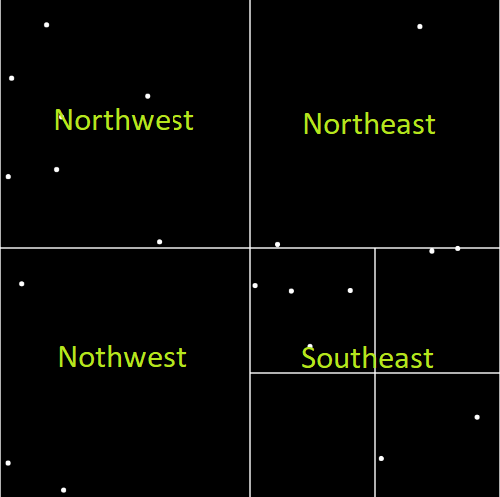
\includegraphics[width=0.6\textwidth]{img/quadtree_cuadrante.png}
	\caption{Disposición de los cuadrantes en el Quadtree}
	\label{fig:quadtree_cuadrante}
\end{figure}

\subsubsection{Resultados de la practica: }

\begin{itemize}
	\item En la figura \ref{fig:quadtree_insert} se puede observar que a medida que se incrementan puntos n $>$ 4 se va subdividiendo el cuadrante en 4 subcuadrantes.
\end{itemize}

\begin{figure}[h!]
	\centering
	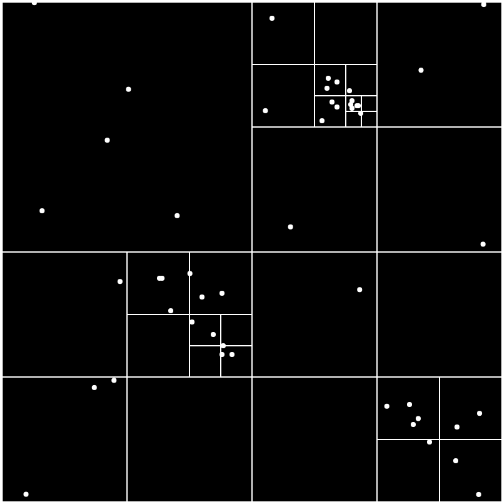
\includegraphics[width=0.6\textwidth]{img/quadtree_insert.png}
	\caption{Inserción de puntos}
	\label{fig:quadtree_insert}
\end{figure}

\begin{itemize}
	\item En la figura \ref{fig:quadtree_insert_data} se puede observar la subdivision de los cuadrantes y los puntos contenidos.
\end{itemize}

\begin{figure}[h!]
	\centering
	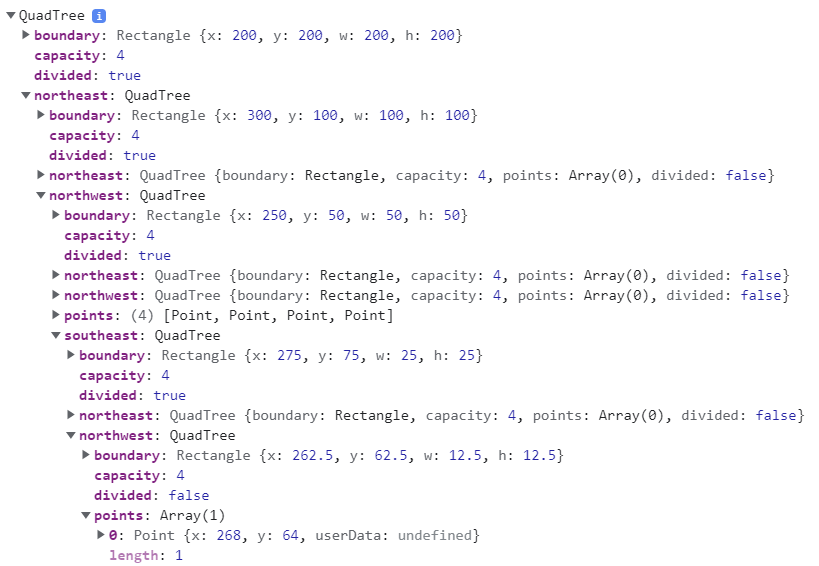
\includegraphics[width=0.9\textwidth]{img/quadtree_insert_data.png}
	\caption{Puntos insertados}
	\label{fig:quadtree_insert_data}
\end{figure}

\begin{itemize}
	\item En la figura \ref{fig:quadtree_search} se puede observar que se van resaltando los puntos dentro del area del cuadro verde, el cual se va intersectando.
\end{itemize}

\begin{figure}[h!]
	\centering
	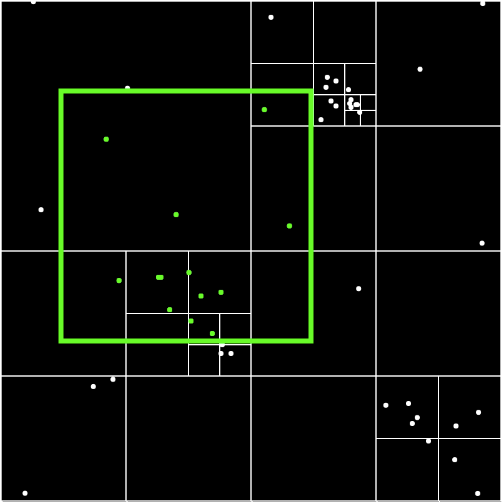
\includegraphics[width=0.6\textwidth]{img/quadtree_search.png}
	\caption{Busqueda de puntos}
	\label{fig:quadtree_search}
\end{figure}
\clearpage
\subsection{Octree}

El Octree es una estructura de datos de árbol en la que cada nodo interno puede tener como máximo 8 hijos. Al igual que el árbol binario que divide el espacio en dos segmentos, Octtree divide el espacio en ocho partes como máximo, lo que se denomina octanos. Se utiliza para almacenar el punto 3-D que ocupa una gran cantidad de espacio. Si todo el nodo interno del Octárbol contiene exactamente 8 hijos, entonces se llama Octárbol completo. También es útil para gráficos de alta resolución como gráficos de computadora en 3D.

El Octree se puede formar a partir de un volumen 3D siguiendo los siguientes pasos de acuerdo a la figura \ref{fig:octree}:

\begin{enumerate}
	\item Divide el espacio 3D actual en ocho cubos.
	\item Si algún cubo tiene más de un punto, divídalo más en 8 cubos.
	\item No divida el cubo que tiene uno o cero puntos
	\item Realice este proceso repetidamente hasta que todo el cuadro contenga uno o cero puntos.
\end{enumerate}
\begin{figure}[h!]
	\centering
	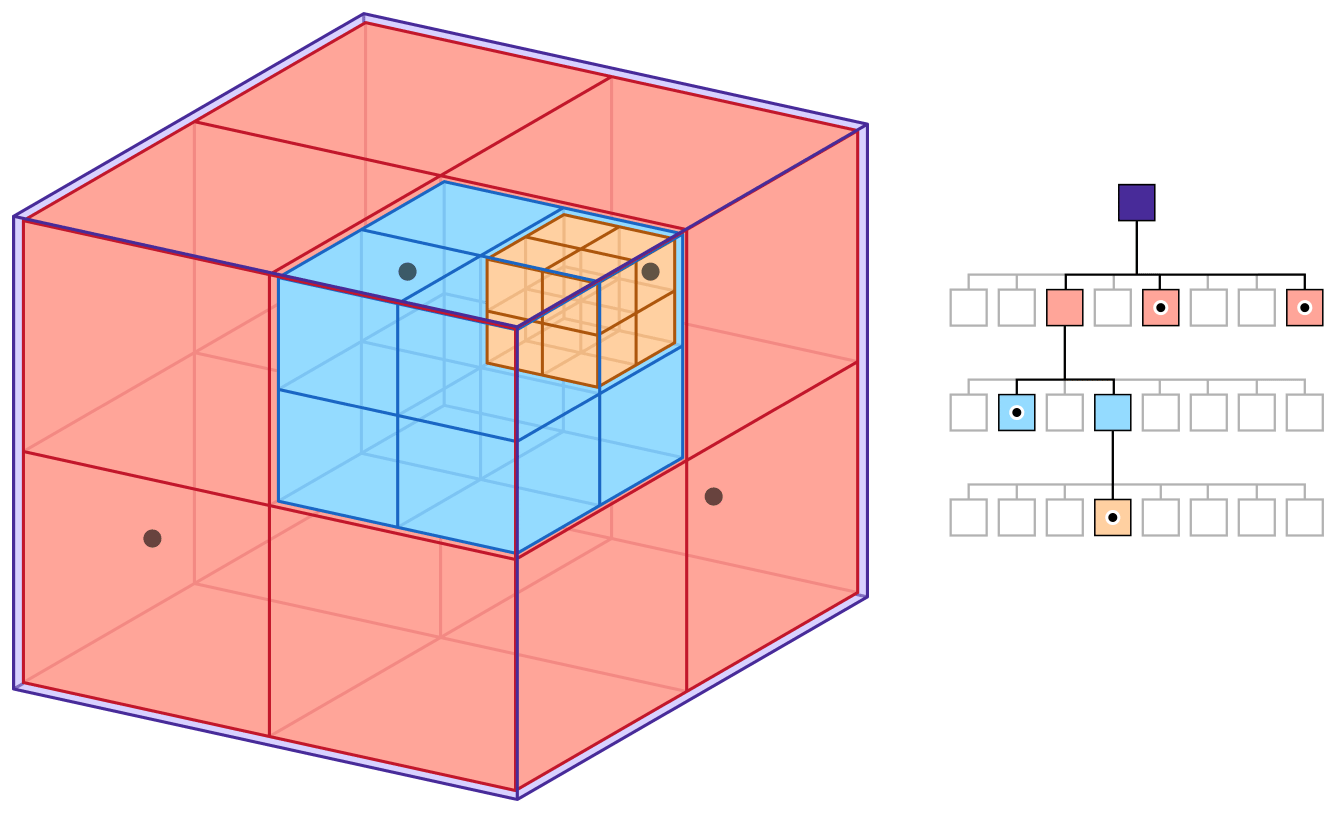
\includegraphics[width=0.8\textwidth]{img/octree.png}
	\caption{Representación gráfica del Octree}
	\label{fig:octree}
\end{figure}

Si S es el número de puntos en cada dimensión, entonces el número de nodos que se forman en Octtree viene dado por esta fórmula (S^{3} -1)/7.

\vspace{5mm}
\textbf{Función Insert:}
\begin{itemize}
	\item Para insertar un nodo en Octree, en primer lugar, verificamos si existe un nodo o no, si existe un nodo, luego regresamos, de lo contrario, vamos recursivamente.
	\item Primero, comenzamos con el nodo raíz y lo marcamos como actual, luego encontramos el nodo secundario en el que podemos almacenar el punto.
	\item Si el nodo está vacío, se reemplaza con el nodo que queremos insertar y convertirlo en un nodo hoja
	\item Si el nodo es el nodo hoja, conviértalo en un nodo interno y si es un nodo interno, vaya al nodo secundario. Este proceso se realiza de forma recursiva hasta que no se encuentra un nodo vacío.
	\item La complejidad temporal de esta función es O(log(N)) donde N es el número de nodos.
\end{itemize}

\textbf{Función Search:}
\begin{itemize}
	\item Esta función se utiliza para buscar el punto existe es el árbol o no.
	\item Comience con el nodo raíz y busque recursivamente si se encuentra el nodo con el punto dado y luego devuelva verdadero, si se encuentra un nodo vacío o un punto límite o un punto vacío, devuelva falso.
	\item Si se encuentra un nodo interno, vaya a ese nodo. La complejidad temporal de esta función también es O(Log N) donde N es el número de nodos
\end{itemize}

\subsubsection{Cuadrantes en Octree: }
\begin{itemize}
	\item Se observa en la figura \ref{fig:octree_cuadrante} como se distrubuyen los cuadrantes en 3D y cuales son los nombres asignados a cada uno de ellos.
\end{itemize}
\begin{figure}[h!]
	\centering
	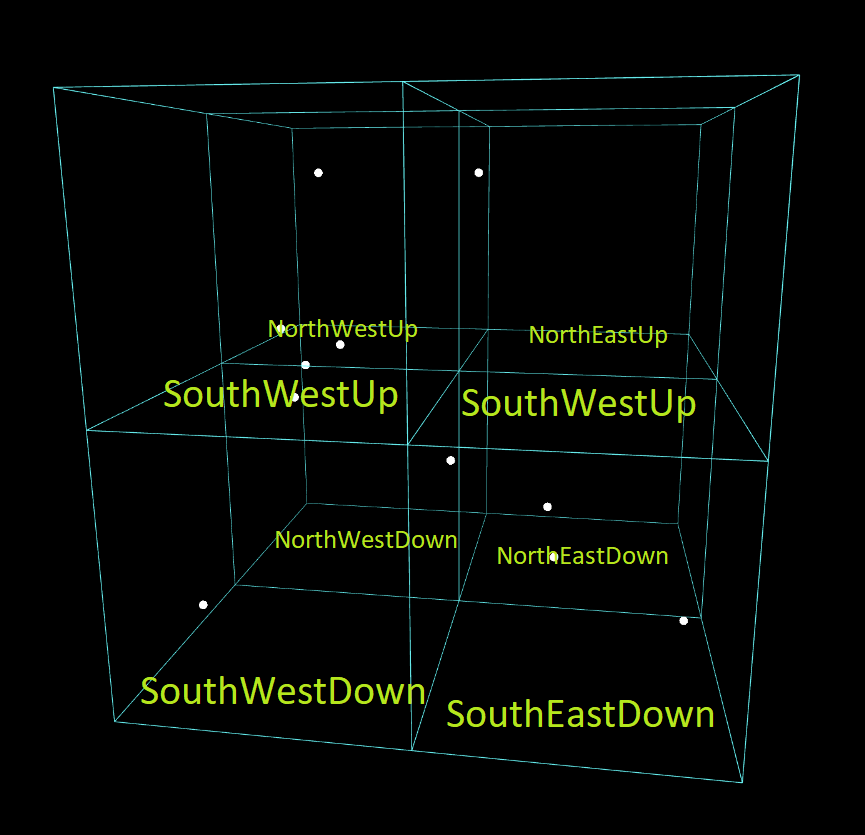
\includegraphics[width=0.6\textwidth]{img/octree_cuadrante.png}
	\caption{Disposición de los cuadrantes en el Octree}
	\label{fig:octree_cuadrante}
\end{figure}
\clearpage
\subsubsection{Resultados de la practica: }

\begin{itemize}
	\item En la figura \ref{fig:octree_insert} se puede observar que a medida que se incrementan puntos n$>$ 2 se va subdividiendo el cuadrante en 8 subcuadrantes.
\end{itemize}

\begin{figure}[h!]
	\centering
	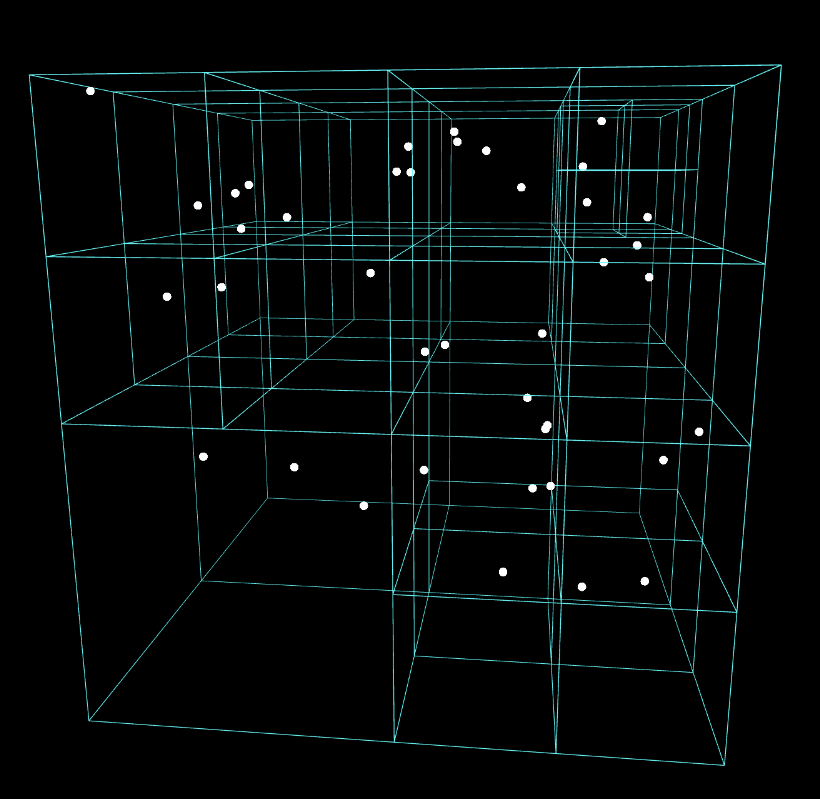
\includegraphics[width=0.6\textwidth]{img/octree_insert.png}
	\caption{Inserción de puntos en octree}
	\label{fig:octree_insert}
\end{figure}
\clearpage
\begin{itemize}
	\item En la figura \ref{fig:octree_insert_data} se puede observar la subdivision de los cuadrantes y los puntos contenidos en cada cuadrante.
\end{itemize}

\begin{figure}[h!]
	\centering
	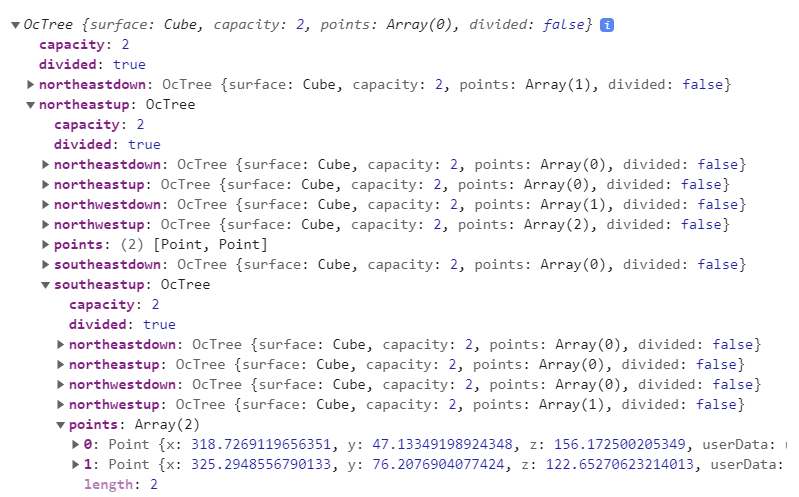
\includegraphics[width=0.9\textwidth]{img/octree_insert_data.png}
	\caption{Puntos insertados en octree}
	\label{fig:octree_insert_data}
\end{figure}


\section{Conclusiones}
\begin{itemize}
	\item El quadtree se codifican en un árbol de cuatro hijos no balanceado, y el  octree se codifica en un árbol octal no balanceado.
	\item De la bibliografía revisada, se concluye que las aplicaciones más comunes para los QuadTree y OcTree son el Procesamiento de imágenes, generación de mallas e indexado espacial.
	\item Las estructuras octree son usadas mayormente para partir un espacio tridimensional, dividiéndolo recursivamente en ocho octantes, siendo análogas tridimensionales de los quadtree bidimensionales.
	\item  El coste medio de insertar un nuevo nodo en un Octree es de O( log 8⁡n), siendo n su número de nodos. Asimismo, el coste por buscar una hoja es O( log 8⁡n).
\end{itemize}
\clearpage
\section{Referencias}
\begin{enumerate}
	\item Tobler, W., & Chen, Z. T. (1986). A quadtree for global information storage. Geographical Analysis, 18(4), 360-371.

	\item Samet, H. (1984). The quadtree and related hierarchical data structures. ACM Computing Surveys (CSUR), 16(2), 187-260.

	\item Rojas Delgado, J. (2015). Estructura de datos espacial jerárquica para la indexación de agrupaciones de objetos geométricos (Bachelor's thesis, Universidad de las Ciencias Informáticas. Facultad 6).

	\item Castillo Oliva, A. D. (2018). Visualización de grandes volúmenes de datos empleando Octree (Bachelor's thesis, Universidad de las Ciencias Informáticas. Centro Vertex, Entornos Interactivos 3D. Facultad 4).

	\item Rivero, J. P. S., de la Hoz, Á. P., & Medina, M. Á. P. GENERACIÓN DE MALLAS APLICACIONES A LA INGENIERÍA.

	\item Brunet Crosa, P., Santisteve i Puyuelo, F., Vilanova, A., Chiarabini, L., Patow, G. A., Staffetti, E., & Surinyac, J. (1999). Estructuras geométricas jerárquicas para la modelización de escenas 3D.

	\item \href{https://p5js.org/es/libraries/}{P5.js}
	\item \href{https://www.geeksforgeeks.org/}{Geeksforgeeks}

\end{enumerate}

\end{document}
